\subsection{Load Management Systems}

A growing number of works on load management systems have primarily focused on industrial load control and have generally ignored the volatility of the energy prices \cite{Gholian7236921, CHEN2015263, Wang6345296, MIDDELBERG20091266}. Most recent works \cite{Sun6329376, DUFLOU2012587, Bakakeu8607483, Pechmann2011} took into account this factor and showed that analytical approaches can be used to compute the optimal time to change the energetic state of a machine for energy control purposes without sacrificing the system throughput. Energy-aware scheduling was also considered to optimize the production plan using mixed integer programming \cite{BRUZZONE2012459, FANG2011234}. However, all the proposed solutions rely on fixed product and machine configurations and thus are not applicable in a dynamic context. Furthermore, these solutions require a precise estimation of the model of the production machine as well as the associated parameters. Since the acquisition of such models mostly rely on expert knowledge, the proposed solutions are not scalable and not cost effective. In this chapter, we focus on a model-free control solution that use RL and do not require an explicit system identification.

\subsection{Reinforcement Learning}
Reinforcement learning (RL) is one of the main classes of machine learning methods that has been successfully applied to solve sequential decision-making problem under uncertainties \cite{Liu6918520}. In such a setting, an agent learns to act using a (partial observable) Markov decision process (MDP) \cite{Sutton9780262039246} formalism. At each time step, the agent selects an action from a finite set of possible actions. After executing the selected action, the environment is updated and the agent receives a rewards signal, which can also be interpreted as a punishment from the environment. The goal of the agent is to maximize the discounted reward in the long run. To achieve this, the agent has to compute the optimal policy based on interactive learning with the environment (see Fig. 1).

% For figures use
%
\begin{figure}[b]
\sidecaption
% Use the relevant command for your figure-insertion program
% to insert the figure file.
% For example, with the graphicx style use
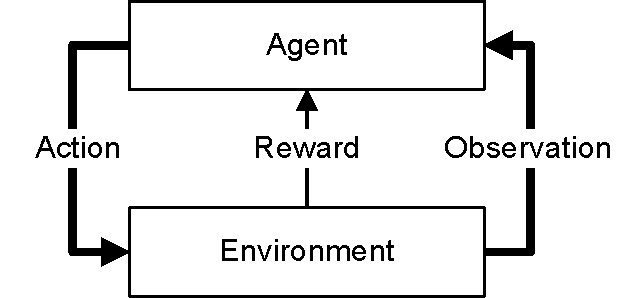
\includegraphics[scale=.65]{images/Single_Agent_RL.pdf}
%
% If no graphics program available, insert a blank space i.e. use
%\picplace{5cm}{2cm} % Give the correct figure height and width in cm
%
\caption{The agent-environment interaction in Reinforcement Learning \cite{Sutton9780262039246}.}
\label{fig:1}       % Give a unique label
\end{figure}


The literature provide many examples of RL algorithms applied to energy management problems. In 1996. Anderson et al. applied Q-learning to modulate the output of the PI controller for a heating coil \cite{ANDERSON1997421, Li6519950}. In the same direction, Ruelens et al.\cite{Ruelens7038106, Ruelens7792709}, De Somer et al. \cite{Somer8260152} and Kazmi et al. \cite{KAZMI2018159} were able to apply RL methods to reduce the domestic water heating costs. Jiang et al. implemented a hierarchical multi-agent Q learning approach for dynamic demand response and distributed energy resource management in a micro-grid \cite{Jiang6912013}. In recent studies \cite{ANVARIMOGHADDAM201741, prasad2018multiagent, LU2018220}, the authors implemented a multi-agent Deep Q-Network (DQN) \cite{mnih2013playing} approach where each agent controlled a house. The agent could consume/store energy, request energy from or grant energy to neighbors, deny energy to neighbors or purchase it from the grid.

\subsection{Multi-Agent Reinforcement Learning}
In multi-agent reinforcement learning (MARL), multiple agents perform concurrently in a single environment \cite{Littman1994multiagent, Hu1998MultiagentRL, Busoniu4445757, Tan93multiagentreinforcement}.  The simplest approach to learning in multi-agent settings is to train each agent independently. This was attempted with Q-learning in \cite{Tan93multiagentreinforcement}, but does not perform well in practice \cite{Matignon2012IndependentRL} since many applications assume interdependency between the agents. More recently, deep neural networks have been successfully used in RL to approximately represent policy and value functions. It is therefore not surprising that deep neural networks have also been applied to MARL settings \cite{tampuu2015multiagent, Gupta71682}, allowing multi-agent learning in high-dimensional/continuous state spaces. However, applying standard RL methods to MARL problems is  challenged by some limitations, such as non-stationary of the environment from the perspective of individual agents \cite{foerster2017stabilising, Lowe2017MultiAgentAF, Foerster2017CounterfactualMP}, lack of coordination/communication in cooperative settings \cite{Lowe2017MultiAgentAF, NIPS2016_6398, MordatchA17, FoersterAFW16a}, credit assignment in cooperative settings with global rewards \cite{Foerster2017CounterfactualMP, Rashid2018,Sunehag3238080}, and the failure to take opponent strategies into account when learning agent policies \cite{He3045581}.

Most relevant to this work are recent approaches \cite{MordatchA17, Foerster2017CounterfactualMP} that propose an actor-critic framework consisting of centralized training with decentralized execution as well as some approaches that utilize attention in a fully centralized multi-agent setting \cite{Choi2017MultifocusAN, Jiang3327828}. The proposed method uses separate centralized critics for each agent, which take all other agent’s actions and observations as input during the training phase, and  actors whose policies are conditioned only on local information. This practice reduces the non-stationary of multi-agent environments, as considering the actions of other agents to be part of the environment makes the state transition dynamics stable from the perspective of one agent. In practice, these ideas greatly stabilize learning because of the reduced variance in the value function estimates.

Our proposed solution follows these recent developments and propose a centralized critic for PPO applied in a multi-agent setting. It is more flexible than the aforementioned approaches in the sense that it is able train policies in environments with any reward setup, observation and action spaces making it broadly applicable to different environment types including industrial micro-grid environments.


